
\chapter{分布式环境下的并行优化工具——star-d}
\label{chap:stard4}

分布式内存下的并行优化的主要优势就是可扩展性较好,但是分布式环境下的编程和调试比共享内存下要复杂的多,因为要考虑复杂的通信和分布式调度算法。但是随着PGAS编程模型的发展,像访问共享内存一样访问分布式内存成为了可能,而且已经有了不少实现了PGAS编程模型的语言和库。star-d的开发就是基于PGAS来实现的,同时任务调度依然采用数据流计算模型。本章下面的内容主要介绍star-d的架构设计、代码实现、API和正确性测试。

\section{选取合适的PGAS实现}

目前已经有许多PGAS的实现,我们需要选取一个合适的PGAS实现,使用它提供的分布式数据结构来简化分布式系统中的通信。选取标准主要有:

\begin{enumerate}
	\item 提供C++ API。
	\item 可以在集群上运行分布式程序。
	\item 便于安装和部署。
\end{enumerate}

经过相关资料的查询,前后共尝试了GPI-2\citep{grunewald2013gaspi}、UPC++\citep{zheng2014upc++}和DASH\citep{furlinger2016dash}这三个PGAS实现,最终选择了DASH作为将要开发的分布式系统的PGAS支持。与之前的调研阶段不同,选取PGAS实现的时候,对每个PGAS实现都在服务器上进行了部署和针对性的测试。下面简要介绍这三个PGAS实现。

\subsection{GPI-2}

GASPI(Global Address Space Programming Interface)\citep{grunewald2013gaspi}是一套PGAS API规范,而GPI 2.0是第一个GASPI标准的实现。经过相关论文的阅读了解到,GPI-2使用单向通信,在性能方面与MPI差不多甚至更加优秀,同时还具有良好的可扩展性、灵活性和容错性。

在集群上部署好GPI后进行了简单的测试,测试结果也正常。接下来基于GPI-2编写了一个C++的测试程序,但是无法编译成功。经过文档的阅读和源代码的检查,发现GPI-2的API是纯C风格的,如果要开发C++版本的程序,必须熟悉GPI-2整个项目的编译规则,然后编译出C++版本的库。由于GPI-2的代码量较大,这个方案可能会非常耗时,不能将主要精力放在分布式系统的架构设计和实现上,所以暂时放弃使用GPI-2,转而寻找其他的PGAS实现。

\subsection{UPC++}

第二个尝试是UPC++,它是UPC的C++扩展,在2017年9月发布。UPC++以C++库的方式提供PGAS支持,其中的许多概念也与GASPI相似,而且用户手册中也有C++版本的测试程序和运行方式。

在集群上部署好UPC++后,运行了一下C++测试程序。在单机上运行多个进程的结果正常,但是在集群上运行分布式程序时出现了错误的结果。在UPC++的文档中也找不到相应的描述,后来经过论文\citep{furlinger2016dash}的阅读发现,UPC++目前还在开发阶段,还没稳定版本的代码,在分布式部署时确实还有一些bug。

\subsection{DASH}

DASH是一个支持PGAS编程模型的C++模板库,而且按照STL的设计方式和概念提供了一些分布式数据结构和并行算法。用DASH编写的程序可以在共享内存或分布式内存环境下运行,它使用异步的单向通信原语处理节点之间的通信。如图4.1是DASH的架构。

\begin{figure}[!htbp]
    \centering
    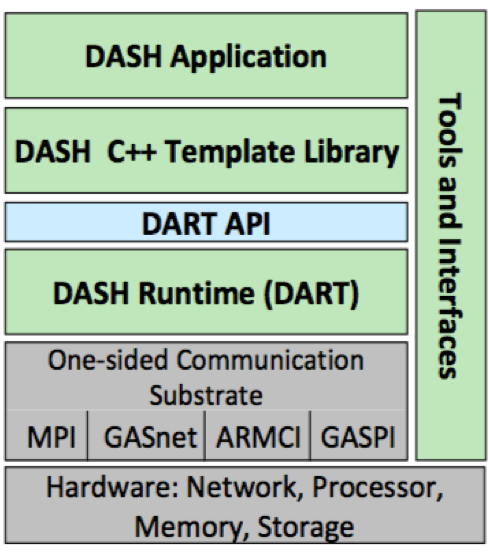
\includegraphics[width=0.40\textwidth]{4_dash_arch}
    \bicaption{DASH的架构。}{Architecture of DASH.}
    \label{fig:4_dash_arch}
\end{figure}
 
通过论文\citep{furlinger2018investigating}的调研,DASH与传统的并行编程和语言(Cilk、TBB、Chapel、Go等)想比,主要的优势有两点:

\begin{enumerate}
	\item 性能优秀:虽然性能不是最高的,但是在各种测试用例上的性能都能取得比较好的成绩。
	\item 开发效率高:首先对于相同的需求,使用DASH开发的程序的代码量较少;其次是代码的可扩展性好,使用DASH开发的同一份代码可以同时在共享内存系统和分布式内存系统上运行,这对开发人员来说是一个极大的便利。
\end{enumerate}

经过文档阅读、集群部署和测试用例的编写,DASH的用例成功的在集群上运行,并且结果符合预期。经过对DASH的编译规则的分析后,成功的运行了自己编写的测试程序。至此到了合适的PGAS实现。

\section{star-d的架构}

\subsection{star-d的总体架构}

\begin{figure}[!htbp]
    \centering
    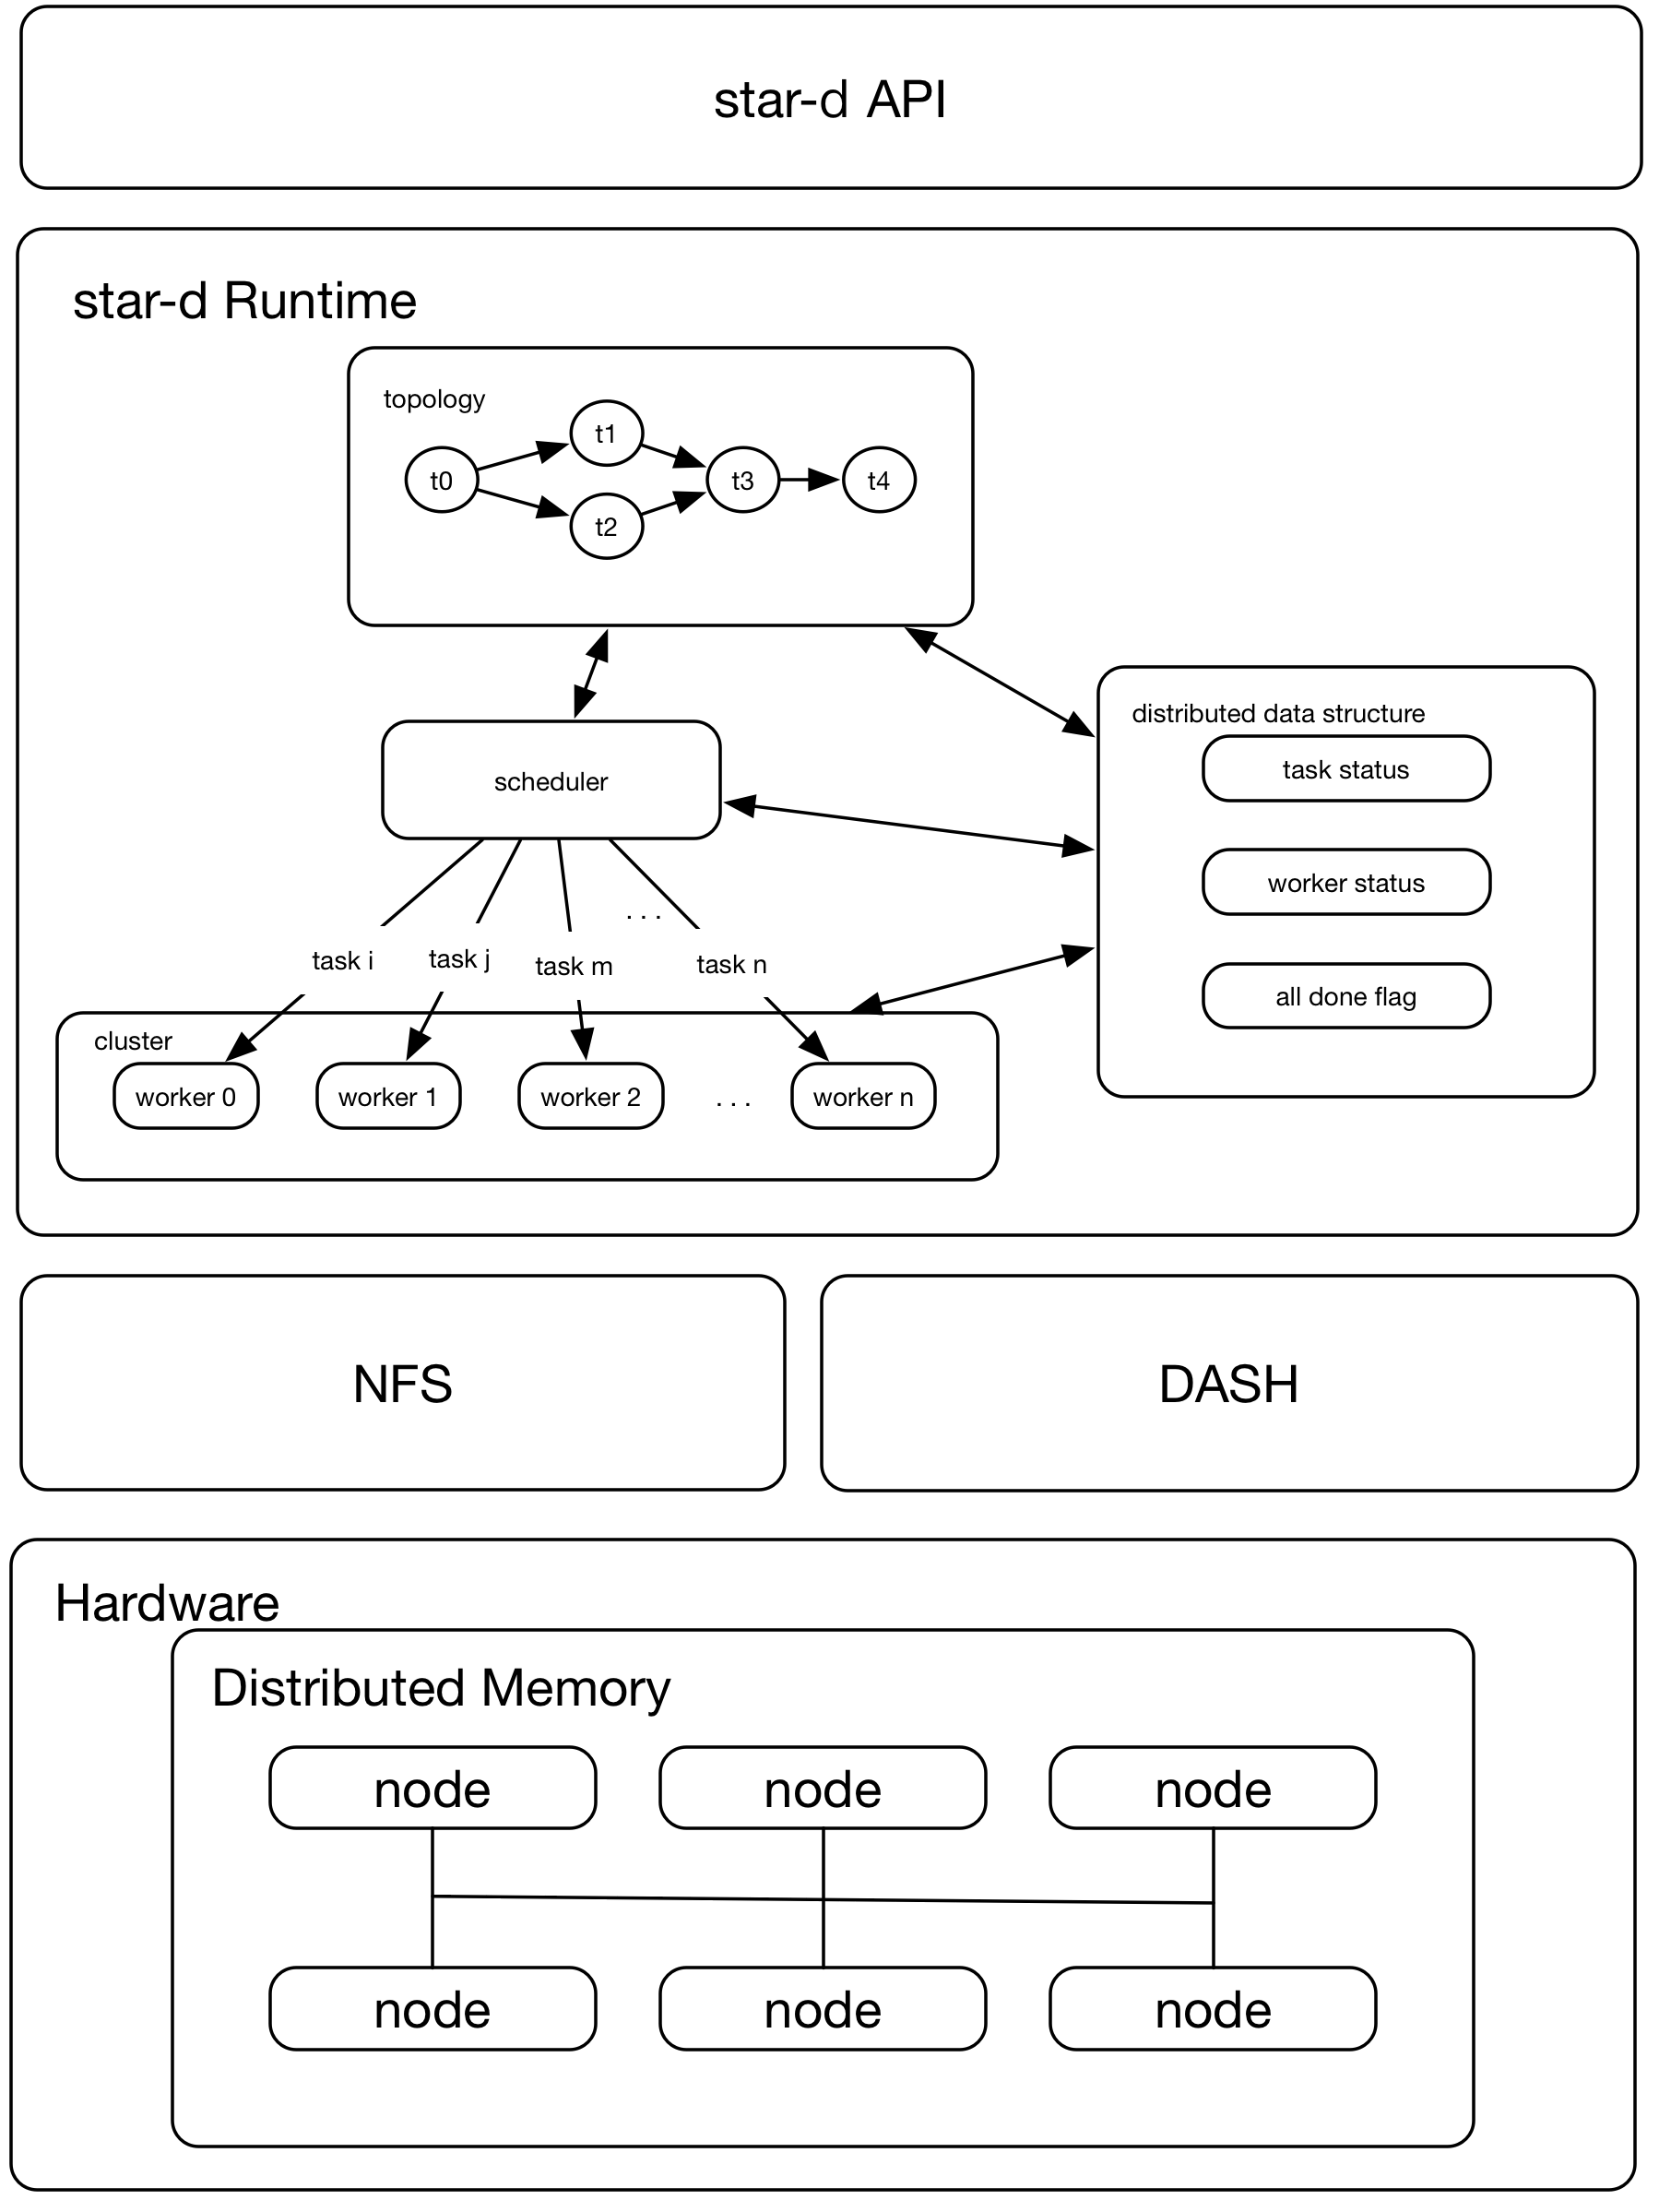
\includegraphics[width=0.40\textwidth]{4_star-d_architecture}
    \bicaption{star-d的总体架构。}{Overall architecture of star-d.}
    \label{fig:4_star-d_architecture}
\end{figure}

如图4.2是star-d的总体架构,自底向上依次包括:

\begin{itemize}
	\item 由多个多核的共享内存节点的组成的分布式集群 (开发和测试的分布式环境包括四个计算节点和一个存储节点 )。
	\item NFS作为分布式文件系统;DASH提供PGAS支持。
	\item star-d的运行时环境:topology和scheduler在master节点上,worker则分布在集群的各个节点上,还有存储task和worker状态的分布式数据结构。
	\item star-d提供的API,主要包括task的定义、topology的建立、scheduler和worker的构建和运行。
\end{itemize}

\subsection{star-d的运行时架构}

\begin{figure}[!htbp]
    \centering
    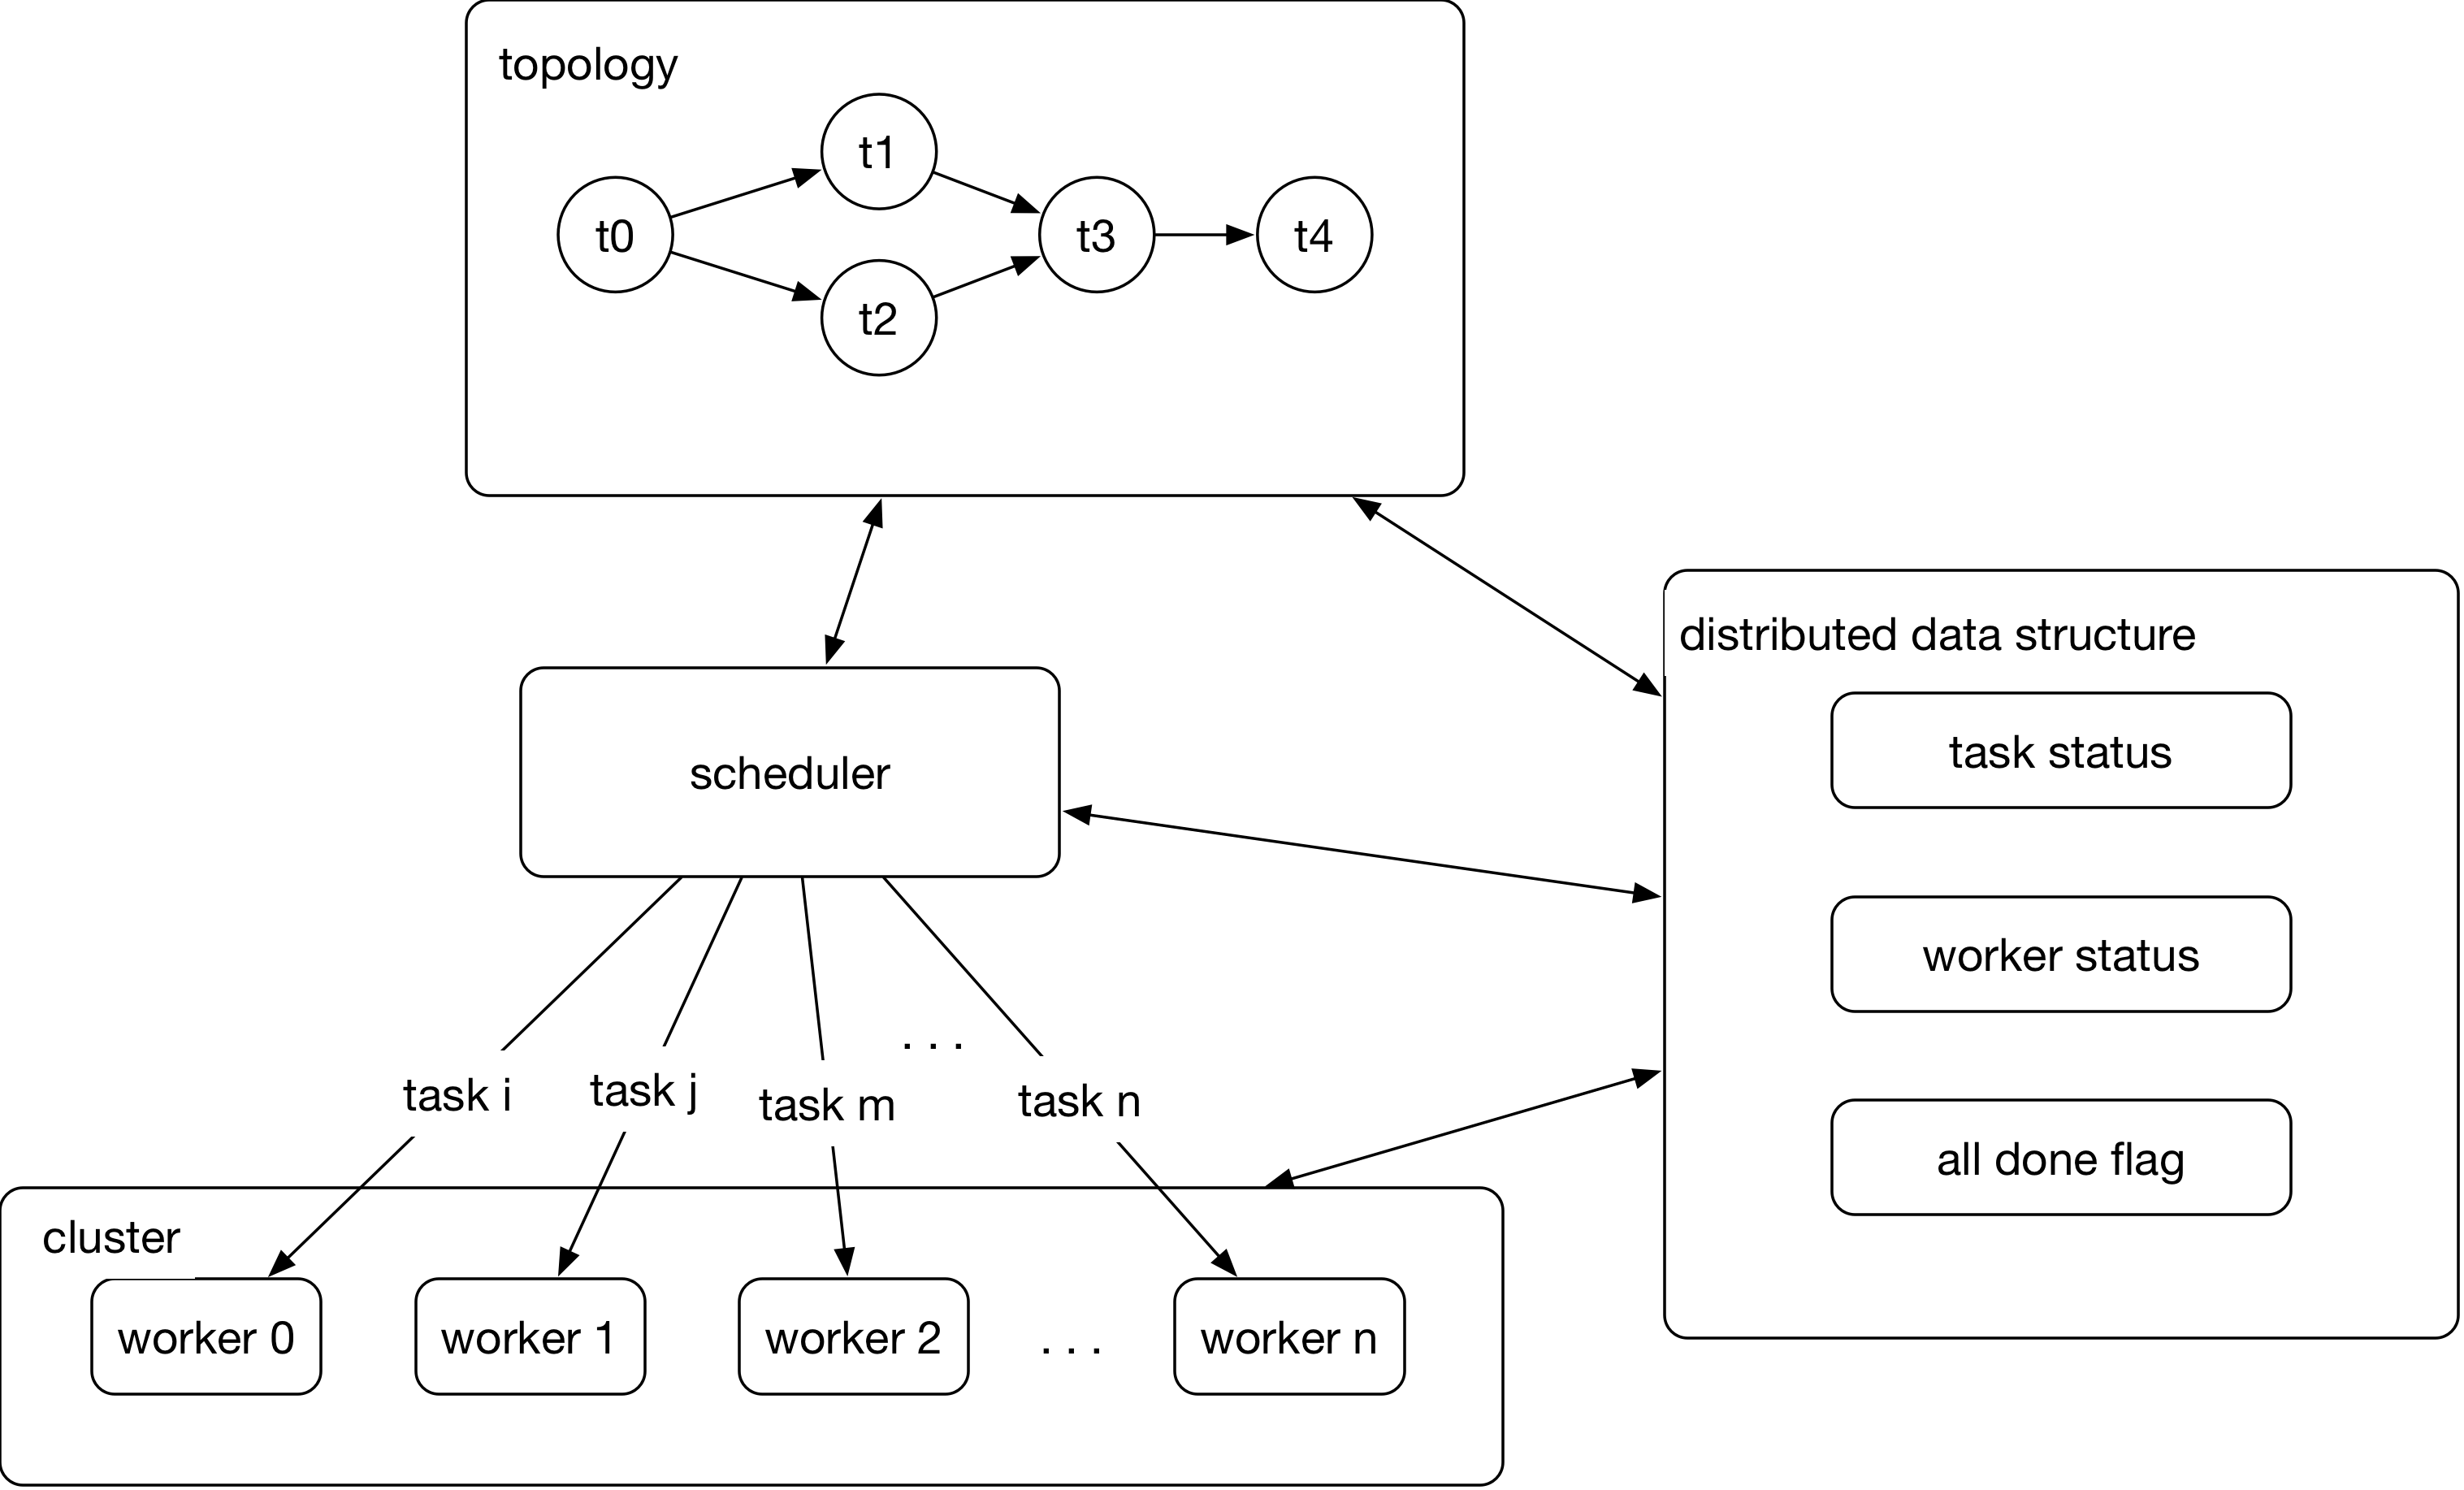
\includegraphics[width=0.80\textwidth]{4_star-d-runtime}
    \bicaption{star-d的运行时架构。}{Runtime architecture of star-d.}
    \label{fig:4_star-d-runtime}
\end{figure}

如图4.3是star-d的运行时架构,主要的模块包括:

\begin{itemize}
	\item topology: 在master进程上运行。缓存task状态,更新task状态和task之间的依赖关系。
	\item scheduler: 在master进程上运行。管理worker的状态,向topology获取就绪任务,将就绪任务分配给空闲的worker。
	\item worker:在每个worker进程上运行。执行scheduler分配的任务。
	\item distributed data structure:scheduler和worker之间通知task和worker的状态。
\end{itemize}

\section{star-d中的任务调度}

star-d中的任务调度同样是master/slave架构:scheduler负责任务的分发;worker负责任务的执行。scheduler和worker共同参与任务状态和worker状态的更新。由于是在分布式内存下,不能像共享内存那样提供线程安全的队列一样构造任务队列。利用DASH提供的分布式数据结构,star-d将任务和worker的状态进行了更加细致的划分,使任务和worker的状态在star-d的运行时环境中保持一致性。

\subsection{star-d中的任务状态}

如图4.4是star-d中的任务状态转换图。

\begin{figure}[!htbp]
    \centering
    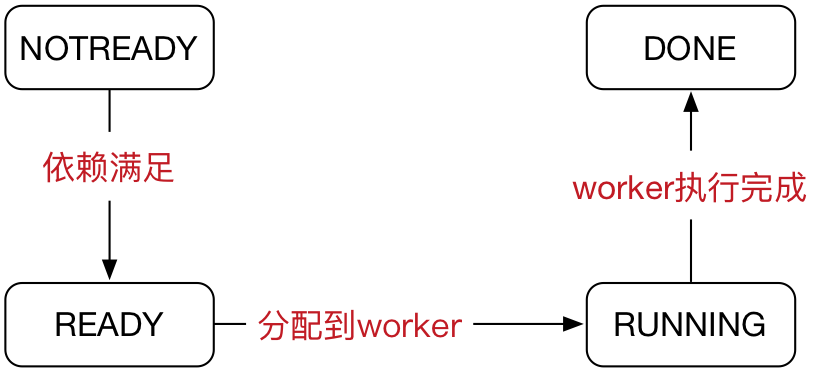
\includegraphics[width=0.50\textwidth]{4_star-d_task_stat}
    \bicaption{star-d中任务状态转换图。}{State transition diagram of tasks in star-d.}
    \label{fig:4_star-d_task_stat}
\end{figure}

star-d中的任务状态包括:

\begin{itemize}
	\item NOTREADY:未就绪。
	\item READY:就绪,尚未分配到worker。
	\item RUNNING:正在运行,已分配给某个worker。
	\item DONE:已完成。
\end{itemize}

\subsection{star-d中的worker状态}

如图4.5是star-d中的worker状态转换图。

\begin{figure}[!htbp]
    \centering
    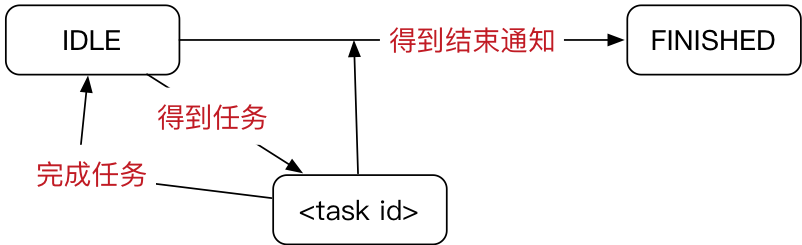
\includegraphics[width=0.50\textwidth]{4_star-d_worker_stat}
    \bicaption{star-d中worker状态转换图。}{State transition diagram of workers in star-d.}
    \label{fig:4_star-d_worker_stat}
\end{figure}

star-d中的worker状态包括:

\begin{itemize}
	\item IDLE:空闲状态,未得到就绪任务。
	\item task id:运行状态,正在执行task id对应的任务。
	\item FINISHED:准备退出状态,执行完当前任务后就退出。
\end{itemize}

\subsection{任务调度策略}

star-d运行时环境初始化后,scheduler会持有所有任务状态的一份拷贝。而且之后更新DAG的过程中,scheduler只在必要的时候才会去访问存储任务状态和worker状态的分布式数据结构。初始化阶段虽然消耗了空间,但是减少了后续调度过程中很多不必要的通信,让调度更加高效。

对于任务状态,未就绪任务的状态存储在集合中,就绪、正在运行和已完成的任务的状态存储在队列中。开始运行后,scheduler安装如4.4所示的状态转换图的方向更新任务的状态。

当有就绪任务(READY状态)时,scheduler就会对worker状态进行轮询,直到找到空闲的worker(IDLE状态),将就绪任务分配给worker,然后将该任务从就绪任务队列出队,并加入到运行任务队列(RUNNING状态) 。

worker执行完一个任务后就会将该任务的状态置为DONE,然后重新将自己的状态置为IDLE,等待下一个任务的到来。

当scheduler更新DAG时,不会考虑未就绪和就绪任务,只需要检查处于RUNNING状态的任务,如果状态已经变为DONE,则放入已完成任务队列,并更新与这个任务相关的依赖关系。当未就绪任务集合中有满足依赖的任务时,就将这个任务移到就绪任务队列中等待被分配并执行。

\section{star-d的API}

\subsection{STask类}

\begin{figure}[!htbp]
    \centering
\begin{lstlisting}[language=c++,caption={}]
class STask {
public:
    explicit STask(std::function<void()> func) : _mFunc(std::move(func)) {}
    ~STask() {}
    void operator()();
    void setId(int);
    int getId();
private:
    std::function<void()> _mFunc;
    int _mId;
};
\end{lstlisting}
    \bicaption{STask类。}{ Class STask.}
    \label{fig:4_stask}
\end{figure}

STask类是star-d中任务的封装,它的定义如图4.6所示。

STask的主要API解释:

\begin{itemize}
	\item 显示构造函数:传入void()类型的函数。
	\item operator()():执行实际的函数。
	\item setId()/getId():设置/获取task id。
\end{itemize}

\subsection{STopology类}

STopology类的定义如图4.7所示,它负责管理所有任务,初始化和更新任务之间的依赖关系等工作。STopology并不为用户提供接口,抽象出topology是为了方便设计scheduler的逻辑。

STopology主要API解释:

\begin{itemize}
	\item 构造函数:传入task列表。
	\item addEdge():添加任务依赖。
	\item size():获取任务个数。
	\item getTask():获取task id对应的任务。
	\item finishAddEdges():完成依赖关系的指定。
	\item updateTaskDependencies():更新任务依赖。
	\item getNextReadyTaskId():获取就绪任务。
\end{itemize}

\begin{figure}[!htbp]
    \centering
\begin{lstlisting}[language=c++,caption={}]
class STopology {
public:
    STopology() : _mSize(0) {}
    STopology(std::vector<STask*>&);
    ~STopology() {}
    void registerTask(STask*);
    void addEdge(STask*, STask*);
    void addEdge(int, int);
    int size();
    STask* getTask(int taskId);
    void finishAddEdges();
    void updateTaskDependencies();
    int getNextReadyTaskId();
    bool isDone();
    bool isTaskDone(int);
    void printAllTaskId();
private:
    int _mSize;
    std::unordered_map<int, STask*> _mIdTaskMap;
    std::vector<std::unordered_set<int>> _mInDeps, _mOutDeps;
    std::unordered_set<int> _mNotReadyTaskIdSet; //, _mDoneTaskIdSet;
    std::queue<int> _mReadyTaskIdQueue, _mRunningTaskIdQueue, _mDoneTaskIdQueue;
};
\end{lstlisting}
    \bicaption{STopology类。}{ Class STopology.}
    \label{fig:4_stopology}
\end{figure}

\subsection{SScheduler类}

\begin{figure}[!htbp]
    \centering
\begin{lstlisting}[language=c++,caption={}]
class SScheduler {
public:
    explicit SScheduler(STopology*, int);
    ~SScheduler() {}
    void run();
private:
    STopology* _mTopology;
    int _mNumWorkers;
    void updateWorkerStat(int);
    int getIdleWorkerId(int);
    void assignTaskToWorker(int, int);
};
\end{lstlisting}
    \bicaption{SScheduler类。}{ Class SScheduler.}
    \label{fig:4_sscheduler}
\end{figure}

SScheduler类的定义如图4.8所示,由于许多调度细节在STopology类中已经解决,SScheduler的逻辑就简明了许多,只需要负责就绪任务的获取和分发,以及worker状态的获取。

SScheduler的主要API解释:

\begin{itemize}
	\item 显示构造函数:传入topology指针和worker的个数。
	\item run():
	\begin{enumerate}
		\item 从topology获取就绪任务。
		\item 获取空闲的worker。
		\item 将就绪任务分配给空闲的worker。
		\item 重复1-3直到所有任务完成。
	\end{enumerate}
\end{itemize}

\subsection{SWorker类}

\begin{figure}[!htbp]
    \centering
\begin{lstlisting}[language=c++,caption={}]
class SWorker {
public:
    explicit SWorker(STopology*, int);
    ~SWorker() {}
    void run();
    void showHistory();
private:
    STopology* _mTopology;
    int _mWorkerId;
    std::queue<int> _mTaskHistory;
};
\end{lstlisting}
    \bicaption{SWorker类。}{ Class SWorker.}
    \label{fig:4_sworker}
\end{figure}

SWorker类的定义如图4.9所示,它负责任务的实际执行,它不断的检查自己的worker状态值,如果状态值是task id,则执行对应的task,执行完后更新task的状态为DONE。

当worker状态值为FINISHED时,表示所有任务已经处于RUNNING或DONE状态,不会再有就绪任务到来,此时,worker就可以退出并打印自己的执行任务历史。

SWorker的主要API解释:

\begin{itemize}
	\item 显示构造函数:传入topology指针和自己的worker id。
	\item run():重复检查自己的worker状态,如果是task id,执行对应的task;如果是FINISHED,退出。
	\item showHistory():打印执行的task的列表。
\end{itemize}

\subsection{SStar模块}

\begin{figure}[!htbp]
    \centering
\begin{lstlisting}[language=c++,caption={}]
namespace star {
void init(int);
void barrier();
void finalize();
int size();
int myid();
} // namespace star
\end{lstlisting}
    \bicaption{SStar模块。}{ SStar module.}
    \label{fig:4_sstar}
\end{figure}

SStar模块如图4.10所示,包括一些star分布式运行时环境的全局函数。

SStar模块的API解释:

\begin{itemize}
	\item init():初始化star运行时环境。
	\item barrier():整体同步,等待所有进程都调用了这个函数后再继续执行。
	\item finalize():退出star运行时环境。
	\item size():开启的进程个数。
	\item myid():当前进程的id。
\end{itemize}

\section{star-d的正确性测试}

star-d的正确性测试用例如图4.11所示。每个节点代表一个任务;每个任务简单的定义为休眠一秒,然后打印task id,箭头代表任务之间存在依赖。

\begin{figure}[!htbp]
    \centering
    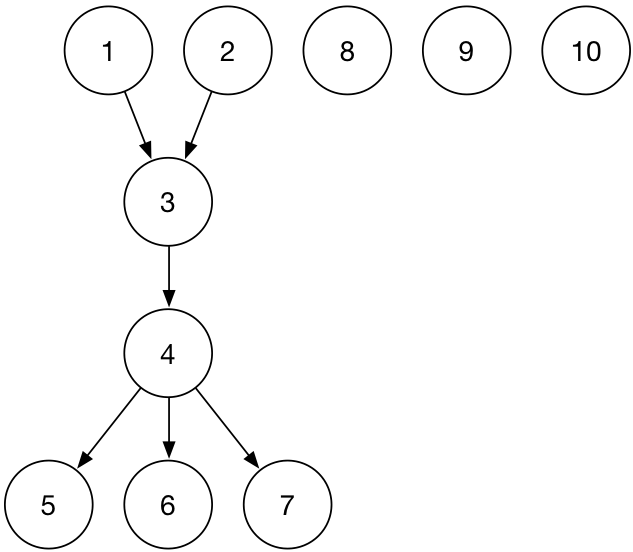
\includegraphics[width=0.40\textwidth]{4_star-d_example_topo}
    \bicaption{star-d测试用例任务拓扑。}{ Task topology of star-d test case.}
    \label{fig:4_star-d_example_topo}
\end{figure}

图4.12中的测试代码对应图4.11的任务拓扑。

star-d测试代码解释:

\begin{itemize}
	\item \textbf{第1行}:待执行函数的定义。
	\item \textbf{第3-6行}:定义STask列表。
	\item \textbf{第7行}:初始化star-d运行时环境。
	\item \textbf{第8-9行}:获取当前进程id和进程总个数。
	\item \textbf{第10-17行}:构造包含所有task信息的topology。
	\item \textbf{第18行}:构造scheduler。
	\item \textbf{第19行}:等待所有初始化过程完成。
	\item \textbf{第20-21行}:开启scheduler和worker。
	\item \textbf{第22行}:退出star-d运行时环境。
\end{itemize}

\begin{figure}[!htbp]
    \centering
\begin{lstlisting}[language=c++,caption={}]
static void func(int i) { sleep(1); printf("task %d\n", i); }
int main(int argc, char* argv[]) {
    vector<star::STask*> tasks;
    tasks.push_back(new star::STask([]{}));
    for (int i = 1; i <= 10; ++i)
        tasks.push_back(new star::STask(std::bind(func, i)));
    star::init(tasks.size());
    int myid = star::myid();
    int size = star::size();
    star::STopology topology(tasks);
    topology.addEdge(1, 3);
    topology.addEdge(2, 3);
    topology.addEdge(3, 4);
    topology.addEdge(4, 5);
    topology.addEdge(4, 6);
    topology.addEdge(4, 7);
    topology.finishAddEdges();
    star::SScheduler scheduler(&topology, size);
    star::barrier();
    if (0 == myid) { scheduler.run();}
    else { star::SWorker(&topology, myid).run(); }
    star::finalize();
    return 0;
}
\end{lstlisting}
    \bicaption{star-d测试代码。}{ Test code of star-d.}
    \label{fig:3_star_tp_example_code}
\end{figure}

运行结果如图4.13所示。运行时指定进行个数为五(一个master,四个worker),指定了mnode01-mnode04四个计算节点。每个worker退出后打印了自己执行任务的历史记录。

\begin{figure}[!htbp]
    \centering
    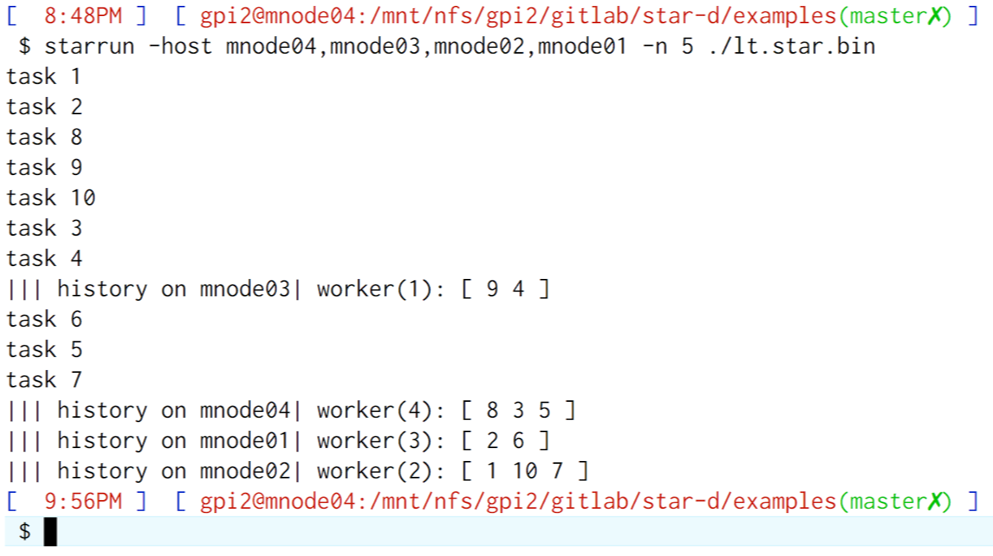
\includegraphics[width=0.60\textwidth]{4_star-d_example_result}
    \bicaption{star-d测试用例运行结果。}{ Result of star-d test case.}
    \label{fig:4_star-d_example_result}
\end{figure}

如表4.1所示,整个运行过程分为四个阶段。

\begin{table}[!htbp]
    \bicaption{star-d测试用例的四个运行阶段。}{Four running phases of star\_tp test case.}
    \label{tab:4_star-d_example_phases}
    \centering
    \footnotesize
    \setlength{\tabcolsep}{4pt}
    \renewcommand{\arraystretch}{1.2} 
    \begin{tabular}{|l|c|}
        \hline
        \bfseries 运行阶段编号 & \bfseries 运行的任务 \\ \hline
        1 & 1,2,8,9\\ \hline
        2 & 3,10\\ \hline
        3 & 4\\ \hline
        4 & 5,6,7\\ \hline
    \end{tabular}
\end{table}

每个阶段的场景还原:

\begin{enumerate}
	\item 程序运行开始后,1、2、8、9、10都是就绪任务,但是只有4个worker,所以1、2、8、9先运行完;
	\item 然后3也ready了,此时只有10和3两个ready的任务,随后10和3执行完;
	\item 3完成后执行4;
	\item 4执行完后,5、6、7都变为ready并且分配给了worker 1、2、3,此时所有任务都处于RUNNING或DONE状态,worker 4变为FINISHED状态,打印执行历史并退出,之后剩下的worker也执行完毕并退出。
\end{enumerate}

这个测试用例一共有10个任务,在4个worker上的执行个数分别为2,3,2,3;如图4.14所示,在另一个有100个任务的测试用例中,在4个worker上的执行个数分别为26,24,26,24。这说明在一定个数的任务个数下,star-d具有一定的负载均衡能力。

\begin{figure}[!htbp]
    \centering
    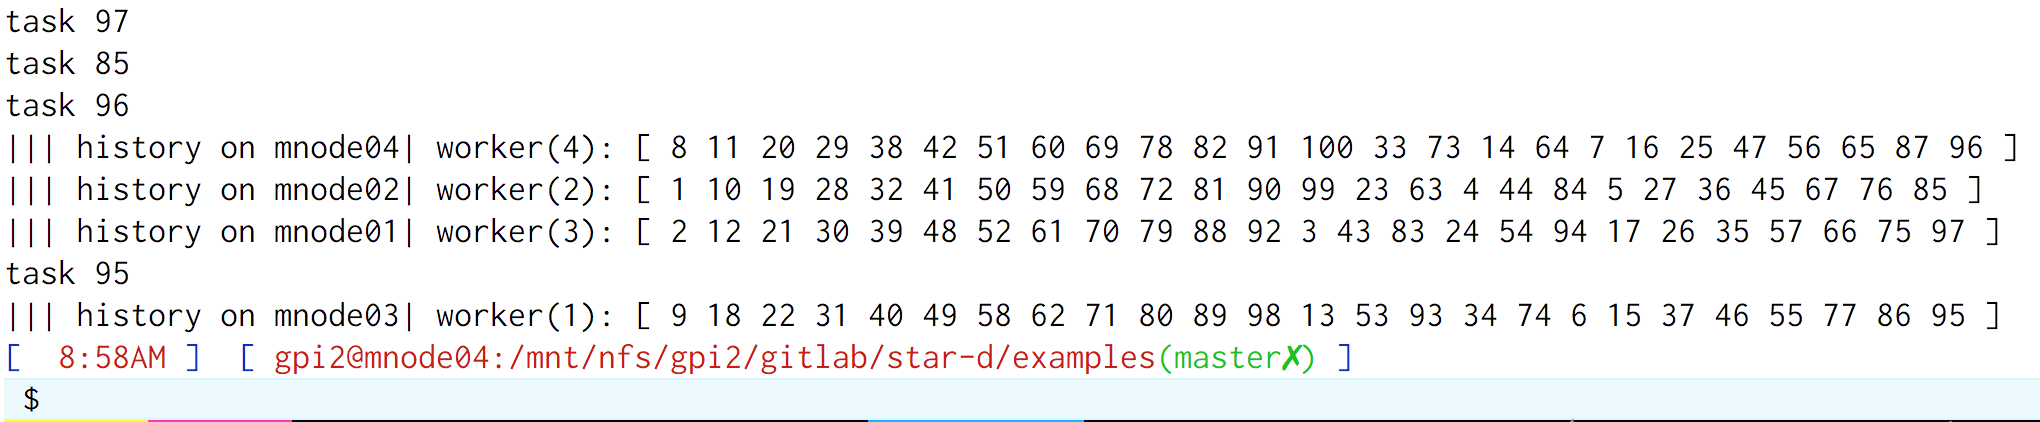
\includegraphics[width=0.60\textwidth]{4_star-d_example_100}
    \bicaption{有100个任务的star-d测试用例运行结果。}{ Result of star-d test case with 100 tasks.}
    \label{fig:4_star-d_example_100}
\end{figure}



